\def \title{bladeRF User Guide}
\def \subtitle{A comprehensive user guide for the Nuand bladeRF}

% Author email and affiliation
\def \emailbpadalino    {\href{mailto:brian.padalino@nuand.com?cc=bladeRF@nuand.com}{\textless{brian.padalino@nuand.com}\textgreater}}
\def \emailjszymaniak   {\href{mailto:jon.szymaniak@nuand.com?cc=bladeRF@nuand.com}{\textless{jon.szymaniak@nuand.com}\textgreater}}
\def \afilnuand         {Nuand, LLC}

% Define authors table
\def \authors{
  \begin{table}[h]
    \centering
    \begin{tabular}{cc}
      Brian Padalino    & Jon Szymaniak     \\
      \emailbpadalino   & \emailjszymaniak  \\
      \afilnuand        & \afilnuand        \\
    \end{tabular}
  \end{table}
}

% Contributors table
%\def \contributors{
%  \begin{table}[h]
%    \centering
%    \begin{tabular}{c}
%    \end{tabular}
%  \end{table}
%}

\def \tablerowcolor{\rowcolor[HTML]{C0C0C0}}
\def \tablecolcolor{\columncolor[HTML]{C0C0C0}}

\def \revisions {
  \begin{table}[h]
    \centering
    \begin{tabular}{|c|c|l|}
      \hline
      \tablerowcolor
      \textbf{Revision} & \textbf{Date} & \textbf{Summary} \hspace{4in}  \\ \hline
      1  & TBD & Draft: Work in progress \\ \hline
    \end{tabular}
  \end{table}
}

% Enable Figure and Table index
\def \enablefiguretableindex{yes}

% Enable acronym list
\def \enableacronymlist{yes}

%-------------------------------------------------------------------------------
%
% This template is a modified version of what is provided at:
%    https://github.com/lungetech/proposal-template
% 
% Copyright (c) 2015, Nuand, LLC
% Copyright (c) 2013, Lunge Technology, LLC
% All rights reserved.
% 
% Redistribution and use in source and binary forms, with or without modification,
% are permitted provided that the following conditions are met:
% 
%   Redistributions of source code must retain the above copyright notice, this
%   list of conditions and the following disclaimer.
% 
%   Redistributions in binary form must reproduce the above copyright notice, this
%   list of conditions and the following disclaimer in the documentation and/or
%   other materials provided with the distribution.
% 
%   Neither the name of the Lunge Technology, LLC nor the names of its
%   contributors may be used to endorse or promote products derived from
%   this software without specific prior written permission.
% 
% THIS SOFTWARE IS PROVIDED BY THE COPYRIGHT HOLDERS AND CONTRIBUTORS "AS IS" AND
% ANY EXPRESS OR IMPLIED WARRANTIES, INCLUDING, BUT NOT LIMITED TO, THE IMPLIED
% WARRANTIES OF MERCHANTABILITY AND FITNESS FOR A PARTICULAR PURPOSE ARE
% DISCLAIMED. IN NO EVENT SHALL THE COPYRIGHT HOLDER OR CONTRIBUTORS BE LIABLE FOR
% ANY DIRECT, INDIRECT, INCIDENTAL, SPECIAL, EXEMPLARY, OR CONSEQUENTIAL DAMAGES
% (INCLUDING, BUT NOT LIMITED TO, PROCUREMENT OF SUBSTITUTE GOODS OR SERVICES;
% LOSS OF USE, DATA, OR PROFITS; OR BUSINESS INTERRUPTION) HOWEVER CAUSED AND ON
% ANY THEORY OF LIABILITY, WHETHER IN CONTRACT, STRICT LIABILITY, OR TORT
% (INCLUDING NEGLIGENCE OR OTHERWISE) ARISING IN ANY WAY OUT OF THE USE OF THIS
% SOFTWARE, EVEN IF ADVISED OF THE POSSIBILITY OF SUCH DAMAGE.
%
%-------------------------------------------------------------------------------

\documentclass[letterpaper,12pt]{article}

\usepackage[printonlyused]{acronym}
\usepackage{amsmath}
%\usepackage[font={small,sf},labelfont={small,sf}]{caption}
\usepackage{float}
\usepackage{caption}
\usepackage{color}
\usepackage{fancyhdr}
\usepackage[includeheadfoot,left=1in,top=.4in,right=1in,bottom=.75in,headsep=\dimexpr3cm-59pt\relax,headheight=59pt]{geometry}
\usepackage{graphicx}
%\usepackage[pagebackref,hyperindex=true]{hyperref}
\usepackage[hidelinks]{hyperref}
\usepackage{listings}
\usepackage{longtable}
\usepackage{mdwlist}
\usepackage{parskip}
\usepackage{setspace}
\usepackage{tabularx}
\usepackage[compact]{titlesec}
\usepackage{xfrac}
\usepackage{xspace}
\usepackage[table,xcdraw]{xcolor}

% default font packages
\usepackage{courier} % use courier for the mono-spaced font 
\usepackage{helvet}  % use a Helvetica clone for default text (sans-serif)

% Uses PDF page rotate attr. Change to lscape if PDF output is not desired.
\usepackage{pdflscape}  

% Drawings
\usepackage[siunitx, american, smartlabels, cute inductors, europeanvoltages]{circuitikz}

%%%
% default document settings
%%%

% setup the default fonts for section headers
\titleformat*{\section}{\sffamily\fontsize{16}{16}\selectfont\bfseries}
\titleformat*{\subsection}{\sffamily\fontsize{14}{14}\selectfont\bfseries}
\titleformat*{\subsubsection}{\sffamily\fontsize{12}{12}\selectfont\bfseries}
\titleformat*{\paragraph}{\sffamily\fontsize{12}{12}\selectfont\bfseries}
\titleformat*{\subparagraph}{\sffamily\fontsize{12}{12}\selectfont\bfseries}

% section numbering
\setcounter{tocdepth}{3}     % display only 3 sections deep in the table of contents
\setcounter{secnumdepth}{5}  % number to 5 sections deep

% add acronyms to the TOC (use chapter, if chapters are available, otherwise use sections
% Based off of suggestions at: http://jevopi.blogspot.com/2009/09/acronyms-and-latex.html
\providecommand{\listofacronymsname}{List of Acronyms and Abbreviations}
\providecommand{\listofacronyms}{
    \ifx\chapter\undefined
        \chapter*{\listofacronymsname}
	    % \addcontentsline{toc}{chapter}{\listofacronymsname}
    \else
        \section*{\listofacronymsname}
		% \addcontentsline{toc}{section}{\listofacronymsname}
    \fi
    \label{sec:acronyms}
	\markboth{\listofacronymsname}{\listofacronymsname}
    \begin{acronym}[AAAAAAAAAAA]
\acro{CPFSK}{Continuous-Phase Frequency Shift Keying}
\acro{CPU}{Central Processing Unit}
\acro{CTCSS}{Continuous Tone-Coded Squelch System}
\acro{CVSD}{Continuously Variable Slope Delta}
\acro{DAC}{Digital to Analog Converter}
\acro{FIR}{Finite Impulse Response}
\acro{FPGA}{Field Programmable Gate Array}
\acro{FRS}{Family Radio Service}
\acro{HDL}{Hardware Description Language}
\acro{IIR}{Infinite Impulse Response}
\acro{GMRS}{General Mobile Radio Service}
\acro{GRC}{GNU Radio Companion}
\acro{GUI}{Graphical User Interface}
\acro{LNA}{Low Noise Amplifier}
\acro{LPF}{Low Pass Filter}
\acro{NBFM}{Narrow-Band Frequency Modulation}
\acro{PLL}{Phase Locked Loop}
\acro{RF}{Radio Frequency}
\acro{RX}{Receive}
\acro{SIB}{Service Indicator Bit}
\acro{SINAD}{Signal-to-Noise and Distoration ratio}
\acro{SDR}{Software Defined Radio}
\acro{TX}{Transmit}
\acro{VCO}{Voltage Controlled Oscillator}
\acro{VGA}{Variable Gain Amplifier}
\acro{VSA}{Vector Signal Analyzer}
\acro{VSG}{Vector Signal Generator}
\end{acronym}

}

%%%
% custom page styles
%%%

\fancypagestyle{plain}{
    \ifdefined\headerleft
      \fancyhead[L]{\headerleft}
    \else
      \fancyhead[L]{}
    \fi
    \ifdefined\headercenter
      \fancyhead[C]{ \textbf{\headercenter}}
    \else
      \fancyhead[C]{ \textbf{\title}}
    \fi
    \fancyhead[R]{ Nuand, LLC}
    \fancyfoot[L]{}
    \fancyfoot[C]{}
    \fancyfoot[R]{\small \thepage}
}

% set the default page style to "plain"
\pagestyle{plain}

%%%
% page templates
%%%

\newcommand{\whitepapercover}{
    \begin{titlepage}
    \thispagestyle{empty}
    \vspace*{1.25in}

    \hfill \textsc{\sffamily\huge\bfseries \MakeLowercase{\title}} \\
    \begin{flushright}
      \ifdefined\subtitle
      \textsc{\sffamily\large \MakeLowercase{\subtitle}} \\
      \vspace*{0.25in}
      \fi
      \textsc{\sffamily\large \MakeLowercase{\today}}
    \end{flushright}

    \vspace{2.5in}
    \begin{center}
        
\includegraphics[width=4.0in]{images/logo.png}
    \end{center}

    \end{titlepage}
    \cleardoublepage
}

\newcommand{\bib}{
    \cleardoublepage
    \pagestyle{plain}
    \phantomsection
    \ifx\chapter\undefined
        \addcontentsline{toc}{chapter}{References}
    \else
        \addcontentsline{toc}{section}{References}
    \fi
    \bibliographystyle{unsrt} % unsrt = plain, except sorted by use, not date.
    {
        \raggedright
        \bibliography{include/refs}
    }
}

\newcommand{\docinfo}{
    \pagenumbering{roman}
    \thispagestyle{plain}
    \section*{License}
    This work by Nuand, LLC is licensed under:
    \begin{center}
      \footnotesize
      \href{http://creativecommons.org/licenses/by/4.0/}{\texttt{Creative Commons Attribution 4.0 International License}} \\
      \vspace{0.125in}
      \href{http://creativecommons.org/licenses/by/4.0/}{
\includegraphics[width=1in]{images/by.png}}
    \end{center}


    \section*{Authors}
    \authors

    \ifdefined\contributors
        \section*{Contributing Authors}
        \contributors
    \fi

    \newpage
    \section*{Revisions}

    Comments, feedback, improvements, and fixes may be sent to \href{mailto:bladeRF@nuand.com}{\textless{bladeRF@nuand.com}\textgreater}.

    \revisions

    \cleardoublepage

    \tableofcontents

    \cleardoublepage

    \ifdefined \enablefiguretableindex
      \listoftables
      \listoffigures
      \cleardoublepage
    \fi

    \ifdefined \enableacronymlist
      \listofacronyms
      \cleardoublepage
    \fi

    \pagenumbering{arabic}
}

%%%
% ease of use macros
%%%

% Example: \q{foo} 
% Results: "foo" - except the quote marks go the right way.
\newenvironment{q}[1]{``#1''} 

% example: C:$\bs$Program Files$\bs$Adobe$\bs$
% Results: C:\Program Files\Adobe\
\def \bs{\char`\\}

% example: \begin{fig}{figure label}{figure caption}{ ... }
% results: A figure, boxed in the center, with font slightly shrunk, with a label and caption
\newcommand{\temporarylabel}{}
\newcommand{\temporarycaption}{}
\newenvironment{fig}[2]{
    \renewcommand{\temporarylabel}{#1}
    \renewcommand{\temporarycaption}{#2}
    \begin{figure}[!htbp]
    \begin{center}
    \begin{small}
}{
    \end{small}
    \end{center}
    \caption{\temporarycaption \label{\temporarylabel}}
    \end{figure}
}

%%%
% Names of products and tool
%
% Use these to ensure capitalization, trademarks, etc., are consistent
% throughout documents.
%%%
\def \tm{\textsuperscript{\textregistered\:}}
\def \windows{Windows\tm}
\def \matlab{MATLAB\tm}
\def \simulink{Simulink\tm}
\def \fx3{FX3\tm}

%%%
% Macros for various conventions
%%%

% Filename
\newcommand{\fname}[1]{\texttt{#1}}
\newcommand{\program}[1]{\texttt{#1}}

%%%
% Styles for code listings
%%%

\definecolor{code-background}{gray}{0.90}
\definecolor{code-comment}{HTML}{005200}

\lstdefinestyle{cmdline}{
    backgroundcolor=\color{code-background},
    frame=single,
    basicstyle=\scriptsize\ttfamily,
    numberstyle=\tiny,
    numbers=left,
    captionpos=b,
    commentstyle=\itshape\color{code-comment},
    keepspaces=true,
    morecomment=[l]{\#},
}


\begin{document}

\whitepapercover
\docinfo

\section{Overview} \label{sec:overview}

This is document provides both architectural and usage information for the
Nuand bladeRF \ac{SDR} \cite{BLADERF}.


\section{Architecture} \label{sec:arch}

The architecture of the bladeRF consists primarily of a LimeMicro LMS6002D RF
transceiver (RF section), an Altera Cyclone IV FPGA (Baseband section), and a
Cypress FX3 USB 3.0 controller (Transport section).

It's recommended to read this section with a copy of the
\href{https://nuand.com/bladerf.pdf}{schematic}\cite{BLADERF_SCHEMATIC}.

\subsection{RF Section} \label{sec:arch-rf}
The RF connections to the bladeRF are two SMA connections RX (J53) and TX (J54).
Each of the RF sections are separated out into a low-band covering 300~MHz
through 1.5~GHz and a high-band covering 1.5~GHz through 3.8~GHz.  The low-band
input goes into RXLNA1 of the LMS6002D whereas the high-band goes into RXLNA2.
The low-band output comes from TXOUT1 and the high-band output comes from
TXOUT2.  Switching between the two bands is accomplished using an AS211-334
SPDT which is controlled by the FPGA.

For reception, internal to the LMS6002D is a zero-IF homodyne receiver
architecture with over 70~dB of variable receive gain, tunable anti-aliasing
filters with bandwidths from 1.5~MHz to 28~MHz, and pair of 12-bit ADCs for
digitizing the baseband signal.  For external observation, header J71 connects
to the analog differential output pins of the LMS6002D.  Pins 1 and 6 connect
to IP and IN, respectively.  Pins 3 and 4 connect to QP and QN, respectively.

\subsection{Baseband Section} \label{sec:arch-bb}
The FPGA is responsible for receiving and transmitting digital baseband samples
as well as command and control of the LMS6002D, Si5338, VCTCXO DAC and RF
switching.

The sample interface on the LMS6002D side is a simple 12-bit interface which
transfers the IQ signal at twice the sample rate.

The command and control interface for the LMS6002D is a 20~MHz SPI connection
which is controlled using a NIOS soft CPU inside the FPGA.

\subsection{Transport Section} \label{sec:arch-transport}
The FX3 is utilized as a transport bridge between the USB connection and the
FPGA.  Samples are communicated over the 32-bit GPIF-II interface whereas
command/control is communicated over the UART.

\subsection{Clocking} \label{sec:arch-clocking}
The bladeRF uses a 1.5~ppm VCTCXO that has a fundamental frequency of 38.4~MHz.
This clock is sent through a 1:2 buffer feeding the FX3 oscillator input as
well as a Silicon Labs Si5338 clock generator.  The Si5338 distributes a
free-running 38.4~MHz clock to the LMS6002D to be used as a frequency reference
and to the Cyclone IV to be used as a system clock.

The Si5338 is also responsible for creating both the TX and RX sampling clocks,
both of which are independent from each other.  The RX clock is fed to the
LMS6002D and fed back to the FPGA to produce a source-synchronous clocked
interface.  The TX clock is considered system-synchronous since the
FPGA is fed a clock with the same phase as the LMS6002D.

The bladeRF is also capable of supplying a clock to the SMB connector at J62.
The purpose of this clock is for distributing a common 38.4~MHz between
multiple devices, or for generating a 10~MHz reference clock to lock external
test equipment to the bladeRF.  The bladeRF cannot accept a 10~MHz input on
J62.

\subsection{Frequency Accuracy} \label{sec:arch-accuracy}
The bladeRF has an on-board 16-bit DAC for fine tuning (trimming) the on-board
VCTCXO.  During factory calibration, the SMB output is fed a buffered 38.4~MHz
clock from the VCTCXO and an external frequency counter is used to measure the
actual frequency.  An algorithm is used to find the DAC value which yields a
measured frequency of 38.4~MHz $\pm 1$~Hz yielding a calibration within 26~ppb.

Due to crystal aging and temperature variation versus calibration, the value
of the DAC may have to change for frequency sensitive setups.


\section{FPGA} \label{sec:fpga}

The FPGA is a very flexible baseband processing element to the bladeRF.
Modifying the FPGA is highly encouraged and welcomed.

\subsection{Building the FPGA Image} \label{sec:fpga-building}
Describe how to build the FPGA image here.

\subsection{Modification} \label{sec:fpga-mods}
The bladeRF Quartus II project is separated into different revisions.  The
preferred method to building a modification is to create and build a new
revision of the FPGA you wanted to modify.

\subsubsection{Adding A New Revision} \label{sec:fgpa-newrev}
Steps to creating a new revision in the project.
Steps for creating the QIP file.
Steps for modification of the source.

\subsection{Clock Domains} \label{sec:fpga-clocks}
The FPGA has four main clock domains: 80~MHz NIOS II clock, 100~MHz GPIF clock,
RX clock, TX clock.  The RX and TX clocks, while they may be the same
frequency, are considered asynchronous to each other due to their unknown
phase relationship.

\subsection{NIOS II Soft CPU} \label{sec:fpga-nios}
The NIOS II Soft CPU inside the FPGA mainly handles command and control of the
bladeRF.  Commands and responses are sent via a UART operating at 4~Mbaud in
an 8-N-1 configuration.

Specifics of the command packet can be found in the software section.

\subsection{GPIF Interface} \label{sec:fpga-gpif}
The GPIF interface is a 32-bit bidirectional interface running at 100~MHz.
This interfaces with the \texttt{fx3\_gpif} block in the FPGA.

For transfers flowing from the FPGA to the GPIF, the FPGA first checks whether
there is enough data for a full DMA transfer.  The DMA transfer size is
determined by the firmware running in the FX3.  By default, each transfer over
the GPIF is 512 32-bit words (2048 bytes) when the USB speed is SuperSpeed, and
256 32-bit words (1024 bytes) when the USB speed is High.  The bladeRF cannot
operate at any other speed.

\begin{center}
    \begin{tikztimingtable}
        [timing/d/background/.style={fill=white}, timing/lslope=0.2]
            PCLK    & L 10{T}         ;[dotted] 4L; 10{T} \\
            RX REQ  & L H 7H H H     ;[dotted] 4H; 5H 5L   \\
            RX ACK  & L L H 6H H H   ;[dotted] 4H; 5H 5L   \\
            DATA    & U U D 6D D D   ;[dotted] 4D; 5D 5U   \\
        \extracode
            \begin{pgfonlayer}{background}
                \begin{scope}[semitransparent,semithick]
                    % \vertlines[gray]{2.1,4.1,...,21.1} % Falling edge
                    \vertlines[gray]{1.1,3.1,...,9.1, 15.1, 17.1,...,23.1} % Rising edge with skip over dot
                \end{scope}
            \end{pgfonlayer}
    \end{tikztimingtable}
\end{center}

Example timing diagram.


\section{Upgrading FX3 Firmware} \label{sec:fw-upgrade}

The firmware executing on the bladeRF's Cypress \fx3 USB peripheral controller
may be updated via a few different methods. Note that there are generally
dependencies between the firmware, the FPGA bitstream, and host software
versions. These dependencies are listed in the bladeRF \fname{CHANGELOG} file
and release notes.

\textit{``Don't Panic!''} It is generally \textbf{not} possible to ``brick'' or damage
the device by accidentally unplugging a device or by closing a program during a
firmware upgrade. In these cases, the \fx3 will enter a recovery bootloader
mode.  Furthermore, it is always possible to force the device into this
recovery state, as detailed in this section.

\subsection{Obtaining Firmware}
Official firmware releases may be obtained from the Nuand webiste: \\
\centerline{\url{https://nuand.com/fx3}}

The following URL always points to the latest available release: \\
\centerline{\url{https://nuand.com/fx3/bladeRF\_fw\_latest.img}}

The remainder of this section assumes the firmware file is named
\fname{bladeRF\_fw\_latest.img} and is located in the current working directory.
Be sure to adjust this accordingly for your specific firmware file and location.

\subsection{Upgrading Firmware via bladeRF-cli}

The \bladerfcli may be used to flash firmware from the command-line 
or in in its interactive mode.

The procedure is as follows:
\begin{enumerate}
    \item Flash new firmware via \bladerfcli.
    \item Power-cycle the device to boot new firmware.
    \item Note the new version number being reported by \bladerfcli.
\end{enumerate}

The commands show in \ref{sec:fw-upgrade-cli} or \ref{sec:fw-upgrade-interactive}
may be used.

\newpage
\subsubsection{Command-line} \label{sec:fw-upgrade-cli}
\begin{lstlisting}[style=numbered-snippet]
$ bladeRF-cli -f bladeRF_fw_latest.img
Flashing firmware...
[INFO @ usb.c:498] Erasing 3 blocks starting at block 0
[INFO @ usb.c:503] Erased block 2
[INFO @ usb.c:511] Done erasing 3 blocks
[INFO @ usb.c:705] Writing 464 pages starting at page 0
[INFO @ usb.c:709] Writing page 463
[INFO @ usb.c:718] Done writing 464 pages
[INFO @ flash.c:110] Verifying 464 pages, starting at page 0
[INFO @ usb.c:603] Reading 464 pages starting at page 0
[INFO @ usb.c:606] Reading page 463
[INFO @ usb.c:617] Done reading 464 pages
Done. A power cycle is required for this to take effect.

# Power cycle device here

$ bladeRF-cli -e version

  bladeRF-cli version:        1.3.1
  libbladeRF version:         1.5.1

  Firmware version:           1.9.0
  FPGA version:               0.5.0
\end{lstlisting}

\subsubsection{Interactive Mode} \label{sec:fw-upgrade-interactive}
\begin{lstlisting}[style=numbered-snippet]
$ bladeRF-cli -i
bladeRF> load fx3 bladeRF_fw_latest.img

  Flashing firmware from bladeRF_fw_latest.img...

[INFO @ usb.c:498] Erasing 3 blocks starting at block 0
[INFO @ usb.c:503] Erased block 2
[INFO @ usb.c:511] Done erasing 3 blocks
[INFO @ usb.c:705] Writing 464 pages starting at page 0
[INFO @ usb.c:709] Writing page 463
[INFO @ usb.c:718] Done writing 464 pages
[INFO @ flash.c:110] Verifying 464 pages, starting at page 0
[INFO @ usb.c:603] Reading 464 pages starting at page 0
[INFO @ usb.c:606] Reading page 463
[INFO @ usb.c:617] Done reading 464 pages
  Done. Cycle power on the device.

bladeRF> quit
$

# Power cycle device here

$ bladeRF-cli -i
bladeRF> version

  bladeRF-cli version:        1.3.1
  libbladeRF version:         1.5.1

  Firmware version:           1.9.0
  FPGA version:               0.5.0

bladeRF> quit
\end{lstlisting}

\newpage
\subsection{Recovering from the Bootloader} \label{sec:recovery}

The \fx3 on the bladeRF falls back to a USB bootloader mode if valid
firmware is not found in SPI flash. In this mode, the device enumerates
with a \texttt{VID:PID = 04b4:00f3}. 

The \cmd{recover} command in \bladerfcli may be used identify
devices in this bootloader state and download firmware to their RAM.

The general recovery procedure, outlined in the remainder of this section is:
\begin{enumerate}
    \item Identify device(s) in bootloader mode
    \item Download and boot firmware from RAM
    \item Write firmware to SPI flash
\end{enumerate}

\subsubsection{Detecting a Device in Bootloader Mode}
When starting up, \bladerfcli detects devices in this bootloader mode
and prints a message alerting users to this: \\

\begin{lstlisting}[style=snippet]
    NOTE: One or more FX3-based devices operating in bootloader mode
          were detected. Run 'help recover' to view information about
          downloading firmware to the device(s).

    No bladeRF device(s) available.
    
    If one is attached, ensure it is not in use by another program
    and that the current user has permission to access it.
\end{lstlisting}

The devices in bootloader mode may be printed using the \cmd{recover} command
with no arguments: \\

\begin{lstlisting}[style=snippet]
bladeRF> recover

  FX3 bootloader devices:
  ---------------------------------------------------------
    Backend:    libusb
    Bus:        1
    Address:    11

  Use 'recover <bus> <addr> <firmware>' to download and boot
  firmware to the specified device.
\end{lstlisting}

\textit{\textbf{Troubleshooting for \windows users}:}
If a device in bootloader mode is not detected, or \bladerfcli fails to open it
via the \cmd{recover} command, it may be the case that \windows is using driver
that is incompatible with \bladerfcli. In this case, one may use \program{Zadig}
 \cite{ZADIG} to install a libusb-compatible driver.

\subsubsection{Downloading Firmware to RAM}
Firmware may be downloaded to the USB peripheral controller's RAM as shown in the
following snippet.  The device will immediately begin executing this firmware,
allowing the device to be opened in \bladerfcli.

{
\noindent\minipage{\linewidth}\medskip
\begin{lstlisting}[style=numbered-snippet]

bladeRF> recover 1 11 bladeRF_fw_latest.img

  Success! Use "open" to switch to this device.
  Note that a "load fx3 <firmware>" is required to write the firmware to flash.

bladeRF> open

bladeRF> info

  Serial #:                 9d1698a25946a1ce2876ab5953b45fb6
  VCTCXO DAC calibration:   0x8ea0
  FPGA size:                40 KLE
  FPGA loaded:              yes
  USB bus:                  2
  USB address:              5
  USB speed:                SuperSpeed
  Backend:                  libusb
  Instance:                 0

bladeRF>
\end{lstlisting}
\endminipage
}

Note that if multiple devices are connected, you may need to provide the
\texttt{-d <device>} arguments to \bladerfcli. \\

\subsubsection{Writing Firmware to SPI Flash}
Firmware executing out of the USB peripheral controller's RAM will not 
persist across power-cycles; it must be written to SPI flash, as exemplified
in Section \ref{sec:fw-upgrade-interactive}. \\

\begin{lstlisting}[style=snippet]
bladeRF> load fx3 bladeRF_fw_latest.img

  Flashing firmware from bladeRF_fw_latest.img...

[INFO @ usb.c:498] Erasing 3 blocks starting at block 0
[INFO @ usb.c:503] Erased block 2
[INFO @ usb.c:511] Done erasing 3 blocks
[INFO @ usb.c:705] Writing 464 pages starting at page 0
[INFO @ usb.c:709] Writing page 463
[INFO @ usb.c:718] Done writing 464 pages
[INFO @ flash.c:110] Verifying 464 pages, starting at page 0
[INFO @ usb.c:603] Reading 464 pages starting at page 0
[INFO @ usb.c:606] Reading page 463
[INFO @ usb.c:617] Done reading 464 pages
  Done. Cycle power on the device.
\end{lstlisting}


\newpage
\subsection{Forcing USB bootloader mode}

There may be situations in which firmware boots from SPI flash, but is
not able to the execute code that allows firmware upgrades to be performed.

This situation might arise if:
\begin{itemize}
    \item A modern libbladeRF version is used in conjunction with a \textit{very} old firmware version
    \item One is developing changes to FX3 firmware and encounters a bug
\end{itemize}

In this situation, it is possible to force the device into its bootloader mode
by placing a jumper across pins 2 and 3 of header \texttt{J64}. This ties one of the
SPI communication to ground, causing SPI flash accesses to fail. As a result, the
device falls back to the bootloader.

\begin{figure}[h]
  \label{fig:j64-jumpered}
  \centering
  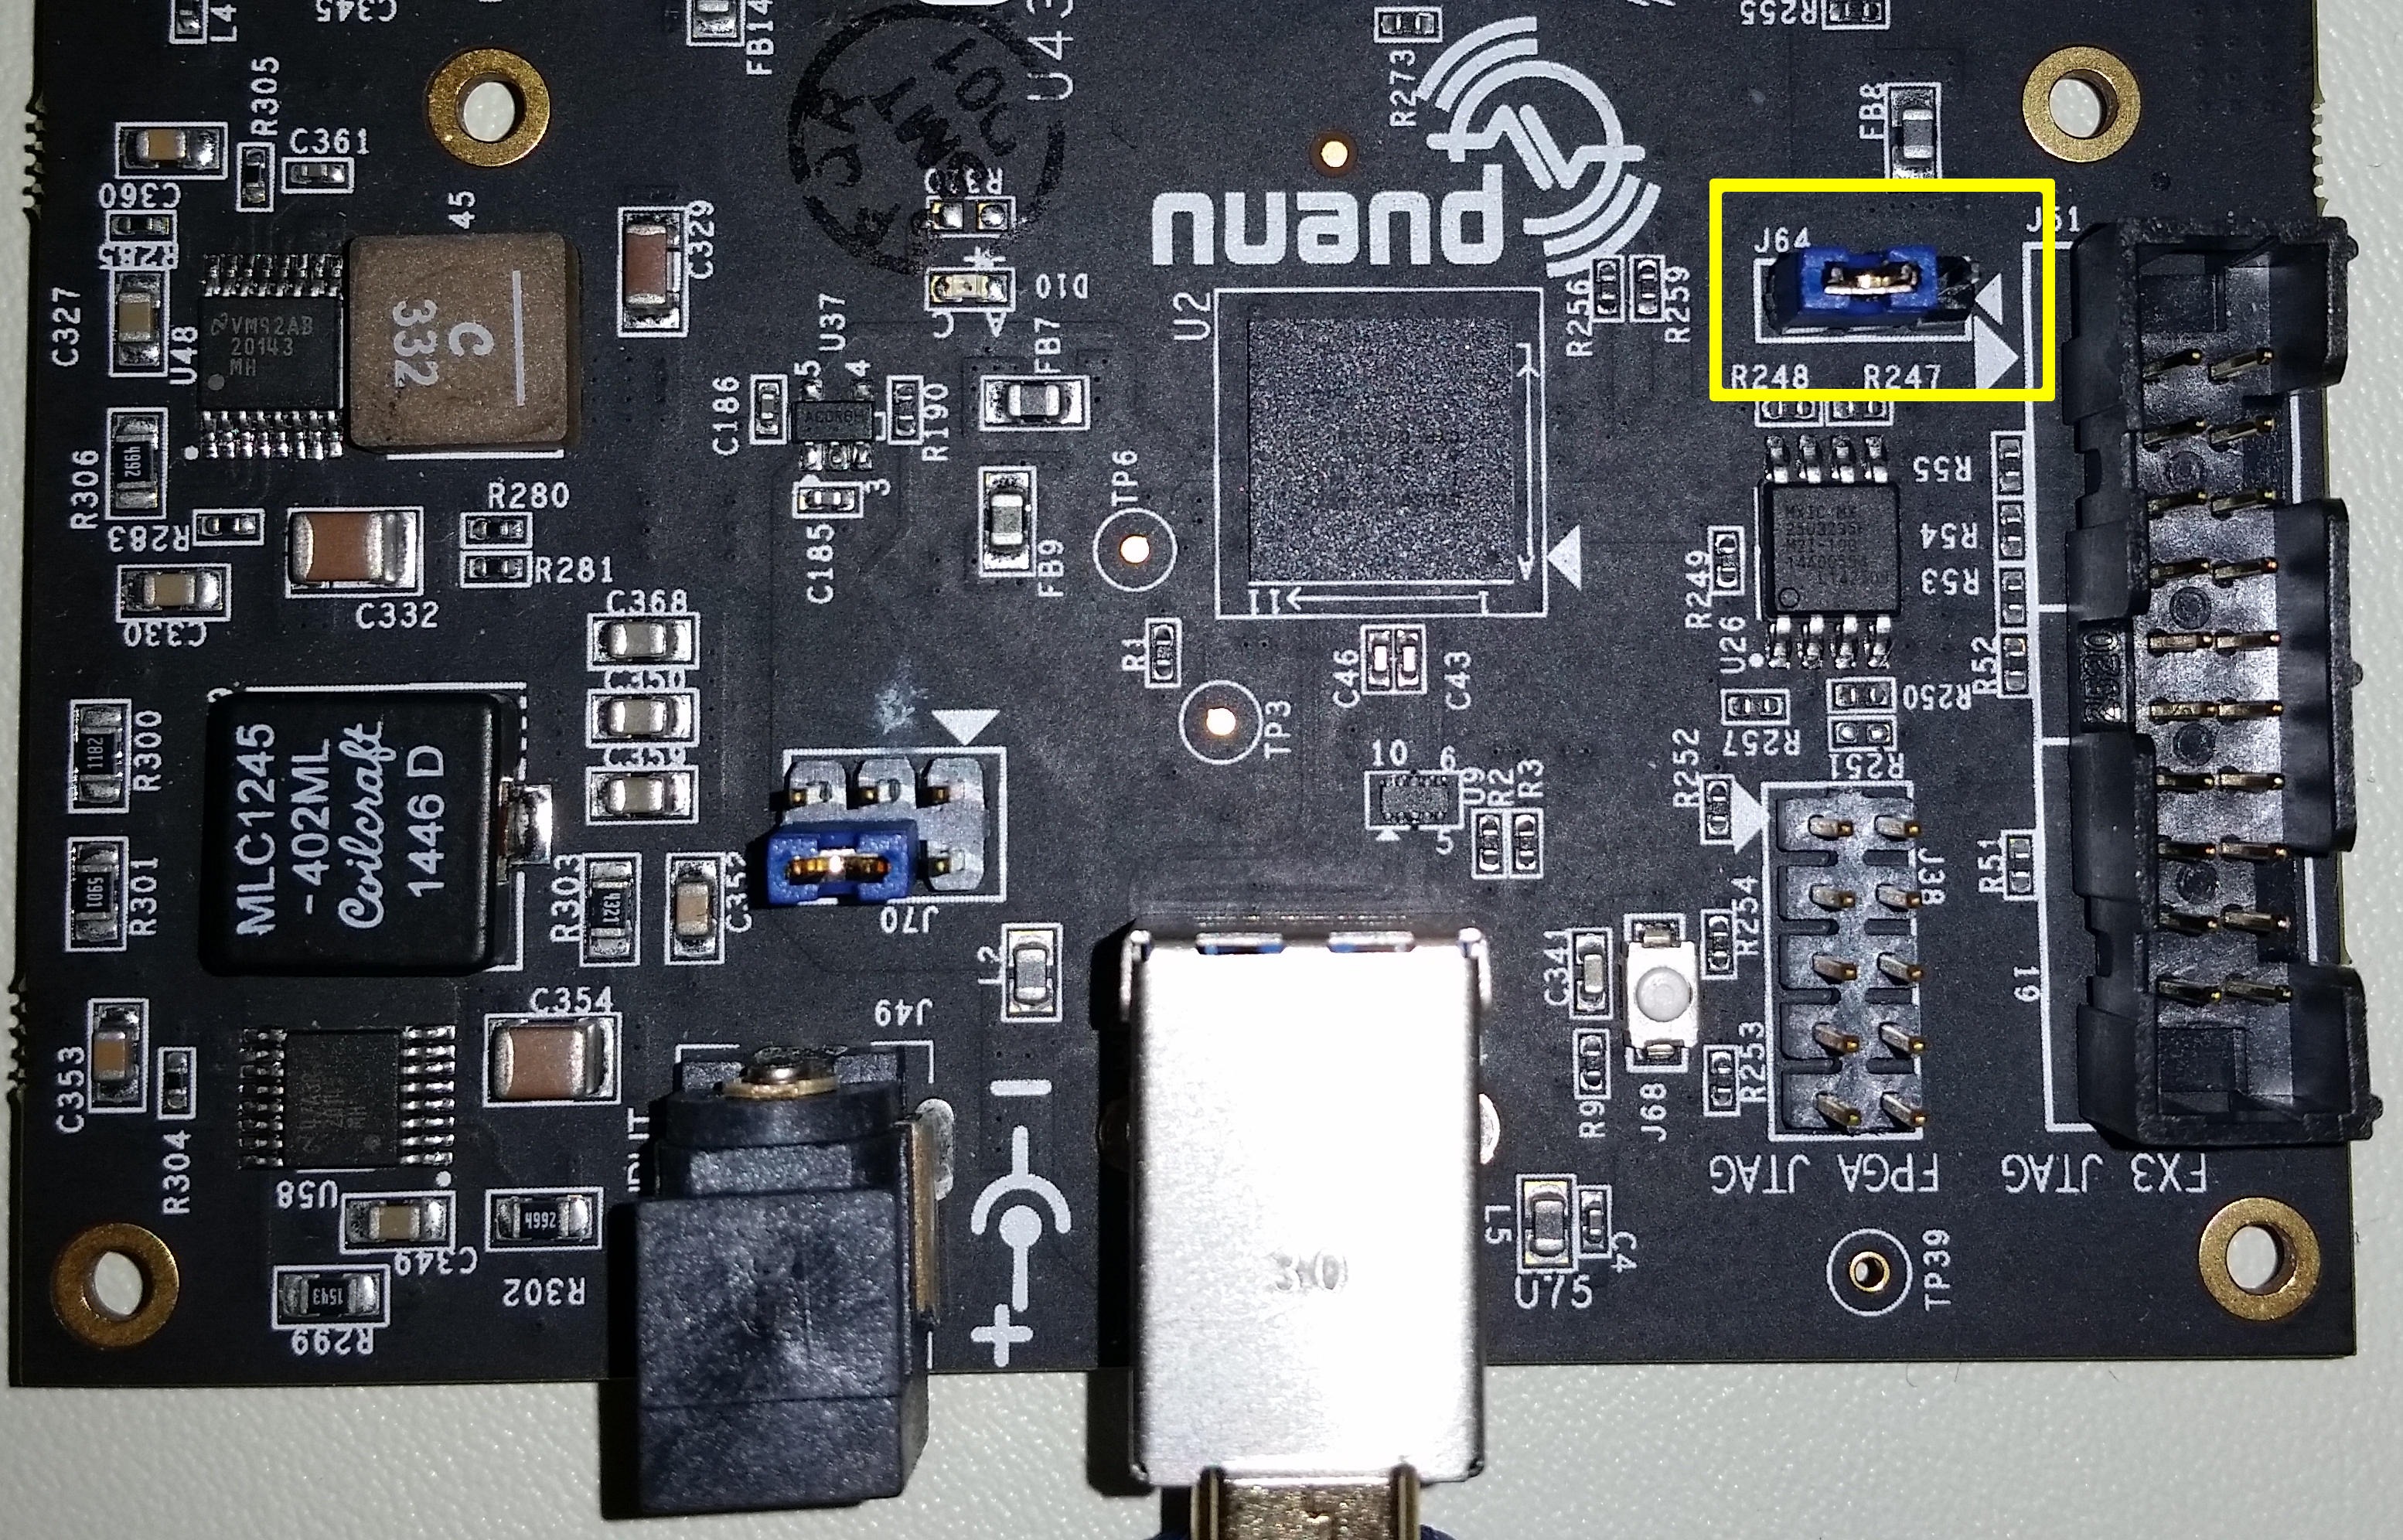
\includegraphics[width=4.5in]{images/bladeRF/j64-jumpered.jpg}
  \caption{bladeRF J64 jumper setting to force bootloader mode}
\end{figure}


To force the device into bootloader mode and re-flash firmware:
\begin{enumerate}
    \item Begin with the bladerf powered off.
    \item Place a jumper across pins 2 and 3 of header \texttt{J64}.
    \item Plug the device in to power it on.
    \item \textbf{Important}: Remove the jumper from \texttt{J64}.
        \begin{itemize}
            \item Forgetting this step will prevent the device from booting firmware in later steps.
        \end{itemize}
    \item Follow Section \ref{sec:recovery} to recover from the bootloader state
\end{enumerate}


\newpage
{\footnotesize \bib}
\end{document}
